\documentclass[letter]{seminar}
\usepackage{calc}               % Simple computations with LaTeX variables
\usepackage[hang]{caption2}     % Improved captions
\usepackage{fancybox}           % To have several backgrounds
                                % (must be loaded before `fancyvrb')
\usepackage{fancyhdr}           % Headers and footers definitions
\usepackage{fancyvrb}           % Fancy verbatim environments
\usepackage{wrapfig}
\usepackage{float}
\usepackage{amsmath}
\usepackage{amssymb}
\usepackage{pdftricks}
\begin{psinputs}
  \usepackage{pstcol}             % PSTricks with the standard color package
                                  % (before `graphicx' for the \scalebox macro)
  \usepackage{graphicx}           % Standard graphics package
  \usepackage{multido}            % General loop macro
  \usepackage{pifont}             % Ding symbols (mainly for lists)
  \usepackage{pst-fr3d}           % PSTricks 3D framed boxes
  \usepackage{pst-grad}           % PSTricks gradient mode
  \usepackage{pst-node}           % PSTricks nodes
  \usepackage{pst-slpe}           % Improved PSTricks gradients
\end{psinputs}
\usepackage{color}
\definecolor{gray}{rgb}{0.5,0.5,0.5}
\definecolor{CodeBorder}{rgb}{0.6,0.6,0.6}
\definecolor{CodeBackground}{rgb}{0.93,0.93,0.93}
\usepackage{graphicx}
\usepackage{fancyvrb}
\usepackage{float}
\usepackage{fvrb-ex}
\usepackage{bold-extra}
\usepackage{ulem}
\usepackage{amssymb,amsmath,epsfig,alltt}
\usepackage{semcolor}           % Seminar colored slides
\usepackage{semhelv}            % Seminar helvetica fonts
\usepackage{semlayer}           % Seminar overlays
\usepackage{slidesec}           % Seminar sections and list of slides
\usepackage{url}                % Convenient URL typesetting
\usepackage[pdftex,letterpaper,pdffitwindow=true,colorlinks=true,pdfpagemode=UseNone,
            bookmarks=true]{hyperref} % Hyperlinks for PDF versions
\usepackage{hcolor}
\slidepagestyle{fancy}

\slidesmag{4}     % Set magnification of slide
\def\SeminarPaperWidth{\paperwidth / 2}
\def\SeminarPaperHeight{\paperheight / 2}
\slideframe{none} % No default frame

  

  % General size parameters
\renewcommand{\slidetopmargin}{-25mm}
\renewcommand{\slidebottommargin}{-10mm}
%  \renewcommand{\slideleftmargin}{4mm}
%  \renewcommand{\sliderightmargin}{4mm}
  % To adjust the frame length to the header and footer ones
%  \autoslidemarginstrue
  % We suppress the header and footer `fancyhdr' rules
\fancyhf{} % Clear all fields
\renewcommand{\headrule}{}
\renewcommand{\footrule}{}

%  \usepackage{nohyperref}       % To deactivate the `hyperref' features
%  \overlaysfalse                % To suppress overlays
%  \def\special@paper{}% Needed to avoid `hyperref' to collapse with ``dvips''
\newslideframe{IMAGE}{%
  \boxput{\rput(0,-9mm){%
      \includegraphics[width=\SeminarPaperHeight,height=\SeminarPaperWidth]{background.pdf}}}{#1}}
\slideframe*{IMAGE}
\RequirePackage[T1]{fontenc}
\RequirePackage{textcomp}
\renewcommand{\rmdefault}{trebuchet}
\renewcommand{\slidefonts}{%
  \renewcommand{\rmdefault}{trebuchet}%
  \renewcommand{\ttdefault}{cmtt}}%
  \newcommand{\ParagraphTitle}[2][black]{%
  \noindent\psshadowbox[fillstyle=solid,fillcolor=#1]{\large{#2}}}
  \newcommand{\CenteredParagraphTitle}[2][black]{%
  \centerline{\psshadowbox[fillstyle=solid,fillcolor=#1]{\large{#2}}}}
  \renewcommand{\makeslideheading}[1]{%
  \CenteredParagraphTitle[black]{%
    \textcolor{black}{\huge\textbf{#1}}}}
  \renewcommand{\makeslidesubheading}[1]{%
    \CenteredParagraphTitle{\Large\theslidesubsection{} -- #1}}
  \renewenvironment{dinglist}[2][black]
  {\begin{list}{\ding{#2}}{}}{\end{list}}
  \newcommand{\DingListSymbolA}{43}
  \newcommand{\DingListSymbolB}{243}
  \newcommand{\DingListSymbolC}{224}
  \newcommand{\DingListSymbolD}{219}
  \newcommand{\eqbox}[2][0.6]{%
  \centerline{\psshadowbox[fillstyle=solid,fillcolor=gray]{%
  \parbox{#1\hsize}{%
      \[
        \textcolor{black} {#2}
      \]}}}}
\renewcommand{\labelitemi}{\footnotesize$\blacktriangleright$}
\renewcommand{\labelitemii}{\footnotesize$\pmb\vartriangleright$}
\renewcommand{\labelitemiii}{$\pmb\rightsquigarrow$}
\begin{document}
\begin{slide}
\begin{center}
\ParagraphTitle{\bf \Large Complete Translation of}
\vspace{5mm} \
{\bf \Large Unsafe Native Code to Safe Bytecode} \\
\vspace{5mm} \
\textit{Brian Alliet, RIT\\Adam Megacz, UC Berkeley} \
\end{center}
\end{slide}

\centerslidesfalse


\begin{slide}\raggedright
\renewcommand{\leftmargini}{5mm}
{\Large{\textcolor{black}{The Problem: Specifics}}}
\\\rule{\textwidth}{0.1pt}\\

\begin{itemize}


\item
     XWT project (pure Java)

\item
     It requires:
\begin{itemize}


\item
         TrueType font rasterization

\item
         {\texttt{.cab}} extraction

\item
         JPEG {\it{decoding}}


\end{itemize}

\end{itemize}


\end{slide}


\begin{slide}\raggedright
\renewcommand{\leftmargini}{5mm}
{\Large{\textcolor{black}{The Problem: Generally}}}
\\\rule{\textwidth}{0.1pt}\\

\begin{itemize}


\item
     Lots of high-quality, complex, code out there in unsafe
      languages
\begin{itemize}


\item
         \TeX

\item
         FreeType

\item
         {\texttt{libjpeg}}

\item
         {\texttt{gcc}}
\end{itemize}


\item
     Need to integrate with Java code

\item
     JNI isn't always an option
\begin{itemize}


\item
         Security

\item
         Portability


\end{itemize}

\end{itemize}


\end{slide}


\begin{slide}\raggedright
\renewcommand{\leftmargini}{5mm}
{\Large{\textcolor{black}{Existing Approaches: Source-to-Source}}}
\\\rule{\textwidth}{0.1pt}\\

\begin{itemize}

\item \begin{figure}[H]
\begin{center}
\epsfig{file=source-to-source,width=\textwidth-1in}
\end{center}
\end{figure}

\end{itemize}


\end{slide}


\begin{slide}\raggedright
\renewcommand{\leftmargini}{5mm}
{\Large{\textcolor{black}{Existing Approaches: Source-to-Source}}}
\\\rule{\textwidth}{0.1pt}\\

\begin{itemize}


\item
         Human-assisted:
\begin{itemize}


\item
             Jazillian

\item
             MoHCA-Java
\end{itemize}


\item
         Partial domain
\begin{itemize}


\item
             {\texttt{c2j}}

\item
             {\texttt{c2j++}}


\end{itemize}

\end{itemize}


\end{slide}


\begin{slide}\raggedright
\renewcommand{\leftmargini}{5mm}
{\Large{\textcolor{black}{Existing Approaches: Source-to-Binary}}}
\\\rule{\textwidth}{0.1pt}\\

\begin{itemize}

\item \begin{figure}[H]
\begin{center}
\epsfig{file=source-to-binary,width=\textwidth-1in}
\end{center}
\end{figure}

\end{itemize}


\end{slide}


\begin{slide}\raggedright
\renewcommand{\leftmargini}{5mm}
{\Large{\textcolor{black}{Existing Approaches: Source-to-Binary}}}
\\\rule{\textwidth}{0.1pt}\\

\begin{itemize}


\item
         {\texttt{egcs-jvm}}

\item
         lcc backend


\end{itemize}


\end{slide}


\begin{slide}\raggedright
\renewcommand{\leftmargini}{5mm}
{\Large{\textcolor{black}{NestedVM: Binary-to-Source}}}
\\\rule{\textwidth}{0.1pt}\\

\begin{itemize}

\item \begin{figure}[H]
\begin{center}
\epsfig{file=binary-to-source,width=\textwidth-1in}
\end{center}
\end{figure}

\end{itemize}


\end{slide}


\begin{slide}\raggedright
\renewcommand{\leftmargini}{5mm}
{\Large{\textcolor{black}{Advantages}}}
\\\rule{\textwidth}{0.1pt}\\

\begin{itemize}


\item
         No modifications to build process

\item
         Language-agnostic

\item
         Bug-for-bug compiler compatability

\item
         Zero post-translation human intervention


\end{itemize}


\end{slide}


\begin{slide}\raggedright
\renewcommand{\leftmargini}{5mm}
{\Large{\textcolor{black}{Why MIPS?}}}
\\\rule{\textwidth}{0.1pt}\\

\begin{itemize}


\item
         Simple, clean, regular semantics

\item
         Well-defined ABI (caller save, callee save)

\item
         Many similarities to JVM
\begin{itemize}


\item
             32-bit aligned memory access

\item
             32x32 => 64bit multiply and divide

\item
             Unsigned math is rare

\item
             Easy to determine likely jump targets


\end{itemize}

\end{itemize}


\end{slide}


\begin{slide}\raggedright
\renewcommand{\leftmargini}{5mm}
{\Large{\textcolor{black}{Memory Representation}}}
\\\rule{\textwidth}{0.1pt}\\

\begin{itemize}

\item \begin{figure}[H]
\begin{center}
\epsfig{file=memory,width=\textwidth-1in}
\end{center}
\end{figure}

\end{itemize}


\end{slide}


\begin{slide}\raggedright
\renewcommand{\leftmargini}{5mm}
{\Large{\textcolor{black}{Code Representation}}}
\\\rule{\textwidth}{0.1pt}\\

\begin{itemize}

\item \vspace{5mm}



\begin{Verbatim}[fontsize=\tiny,frame=single,rulecolor=\color{CodeBorder},resetmargins=true,gobble=0]
private final static int r0 = 0;
private int r1, r2, r3, /* ... */ r30;
private int r31 = 0xdeadbeef;

public void run() {
    while (true)
        switch(pc) {
            case 0x10000: r29 = r29 - 32;
            case 0x10004: r1 = r4 + r5;
            case 0x10008: if (r1 == r6) {
                            /* delay slot */
                            r1 = r1 + 1;
                            pc = 0x10018:
                            continue; }
            case 0x1000C: r1 = r1 + 1;
            case 0x10010: r31 = 0x10018;
                          pc = 0x10210;
                          continue;
            case 0x10014: /* nop */
            case 0x10018: pc = r31; continue;
\end{Verbatim}


\end{itemize}


\end{slide}


\begin{slide}\raggedright
\renewcommand{\leftmargini}{5mm}
{\Large{\textcolor{black}{Trampoline Insertion}}}
\\\rule{\textwidth}{0.1pt}\\

\begin{itemize}

\item \vspace{5mm}



\begin{Verbatim}[fontsize=\tiny,frame=single,rulecolor=\color{CodeBorder},resetmargins=true,gobble=0]
public void run_0x10000() {
    while (true) switch(pc) {
        case 0x10000: ...
        case 0x10004: ...
        case 0x10010: r31 = 0x10018;
                      pc = 0x10210;
                      continue;
....

pubic void run_0x10200() {
    while (true) switch(pc) {
        case 0x10200: ...
        case 0x10204: ...
....

public void trampoline() {
    while (true) switch(pc&0xfffffe00) {
        case 0x10000:    run_0x10000(); break;
        case 0x10200:    run_0x10200(); break;
        case 0xdeadbe00: ...
\end{Verbatim}


\end{itemize}


\end{slide}


\begin{slide}\raggedright
\renewcommand{\leftmargini}{5mm}
{\Large{\textcolor{black}{Binary-to-Binary Translation}}}
\\\rule{\textwidth}{0.1pt}\\

\begin{itemize}

\item \begin{figure}[H]
\begin{center}
\epsfig{file=binary-to-binary,width=\textwidth-1in}
\end{center}
\end{figure}

\end{itemize}


\end{slide}


\begin{slide}\raggedright
\renewcommand{\leftmargini}{5mm}
{\Large{\textcolor{black}{Binary-to-Binary Translation}}}
\\\rule{\textwidth}{0.1pt}\\

\begin{itemize}


\item
         Allows the use of more optimal bytecode sequences that cannot be expressed 
          in java source

\item
         Smaller Bytecode - Javac doesn't emit space efficient bytecode

\item
         Translation is Much faster - doesn't need to go though the extra java
          source compilation step

\item
         Compiled code can be loaded into the JVM at Runtime.


\end{itemize}


\end{slide}


\begin{slide}\raggedright
\renewcommand{\leftmargini}{5mm}
{\Large{\textcolor{black}{Binary-to-Binary: Performance}}}
\\\rule{\textwidth}{0.1pt}\\

\begin{itemize}

\item \begin{figure}[H]
\begin{center}
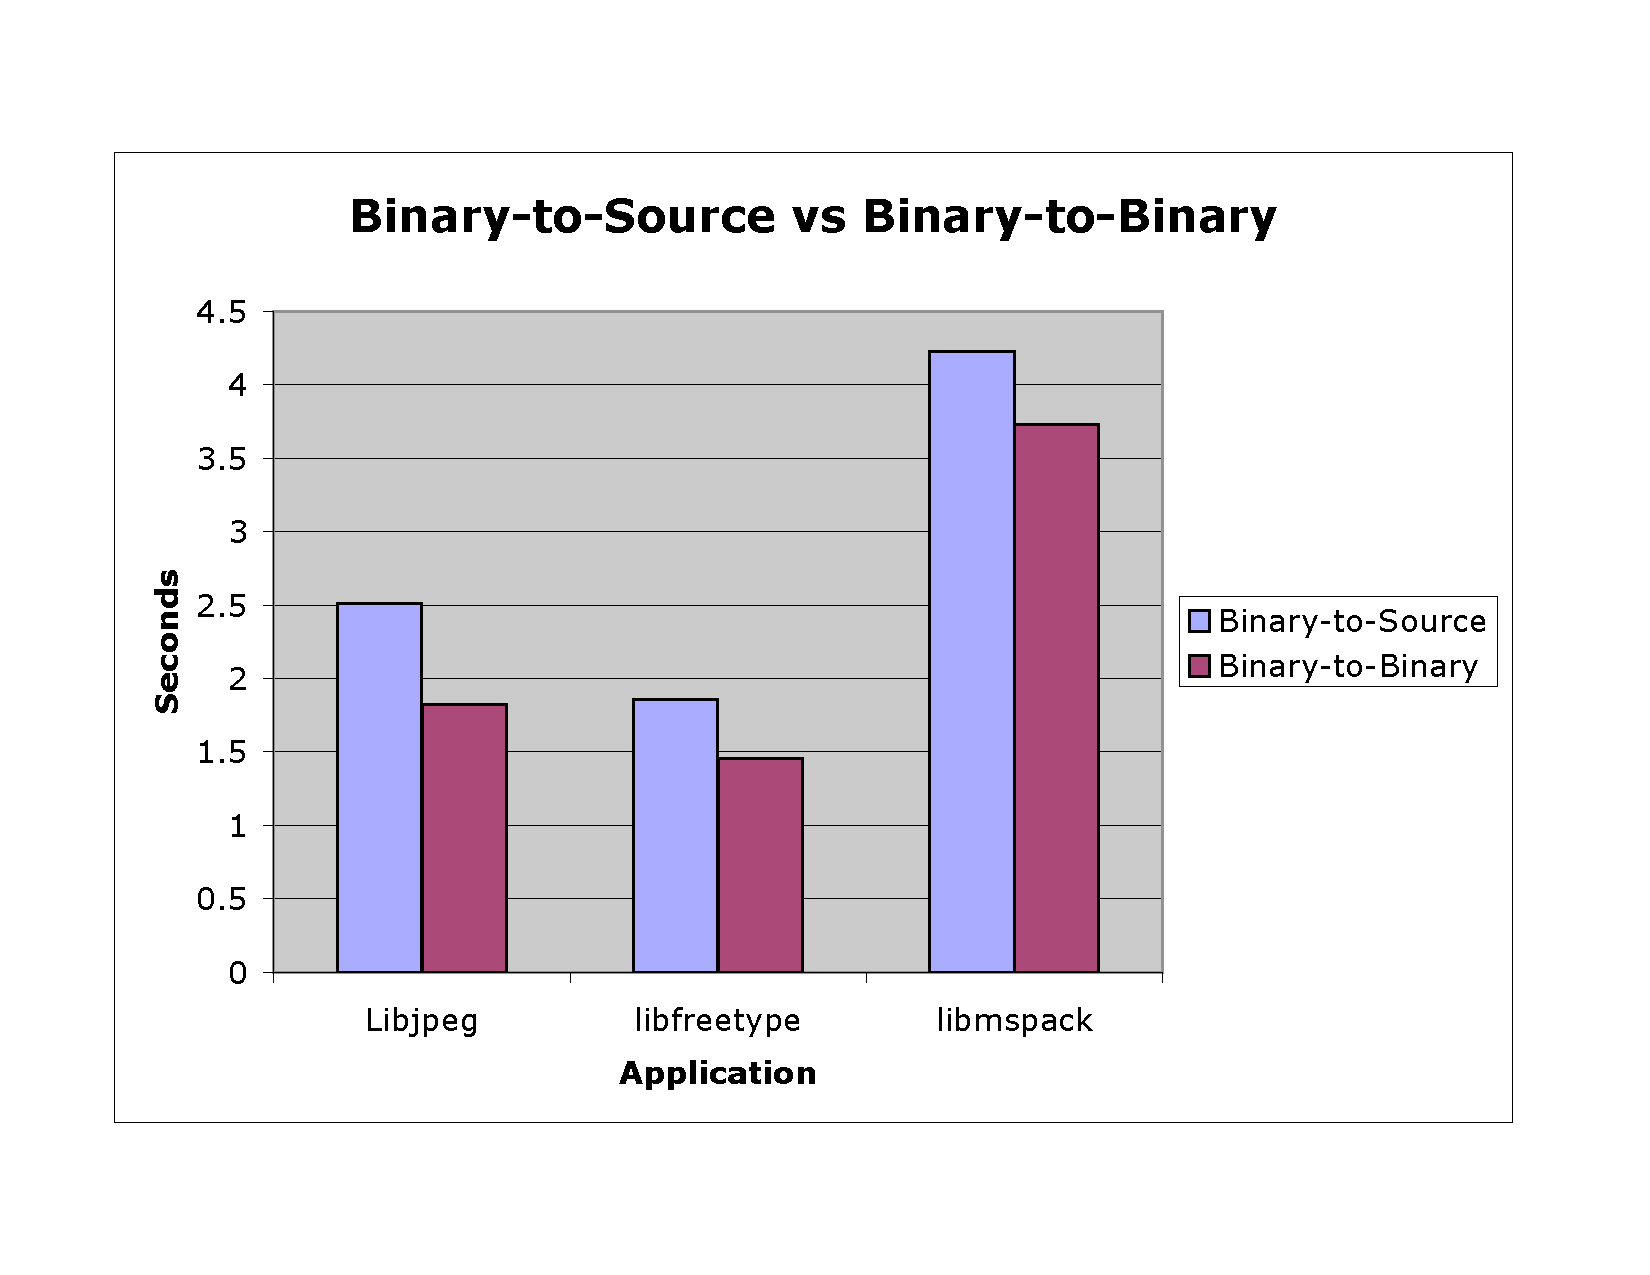
\epsfig{file=chart7,width=\textwidth-1in}
\end{center}
\end{figure}

\end{itemize}


\end{slide}


\begin{slide}\raggedright
\renewcommand{\leftmargini}{5mm}
{\Large{\textcolor{black}{Binary-to-Binary: Performance}}}
\\\rule{\textwidth}{0.1pt}\\

\begin{itemize}


\item
        Performance increased from 10-30\%  after compiling to bytecode 
         directly

\item
        Increase was primarily the result of two things
\begin{itemize}


\item
            More optimal handing of branch instructions

\item
            Use if the JVM stack in favor of temporary variables


\end{itemize}

\end{itemize}


\end{slide}


\begin{slide}\raggedright
\renewcommand{\leftmargini}{5mm}
{\Large{\textcolor{black}{Optimizations: Optimal Method Size}}}
\\\rule{\textwidth}{0.1pt}\\

\begin{itemize}

\item \begin{figure}[H]
\begin{center}
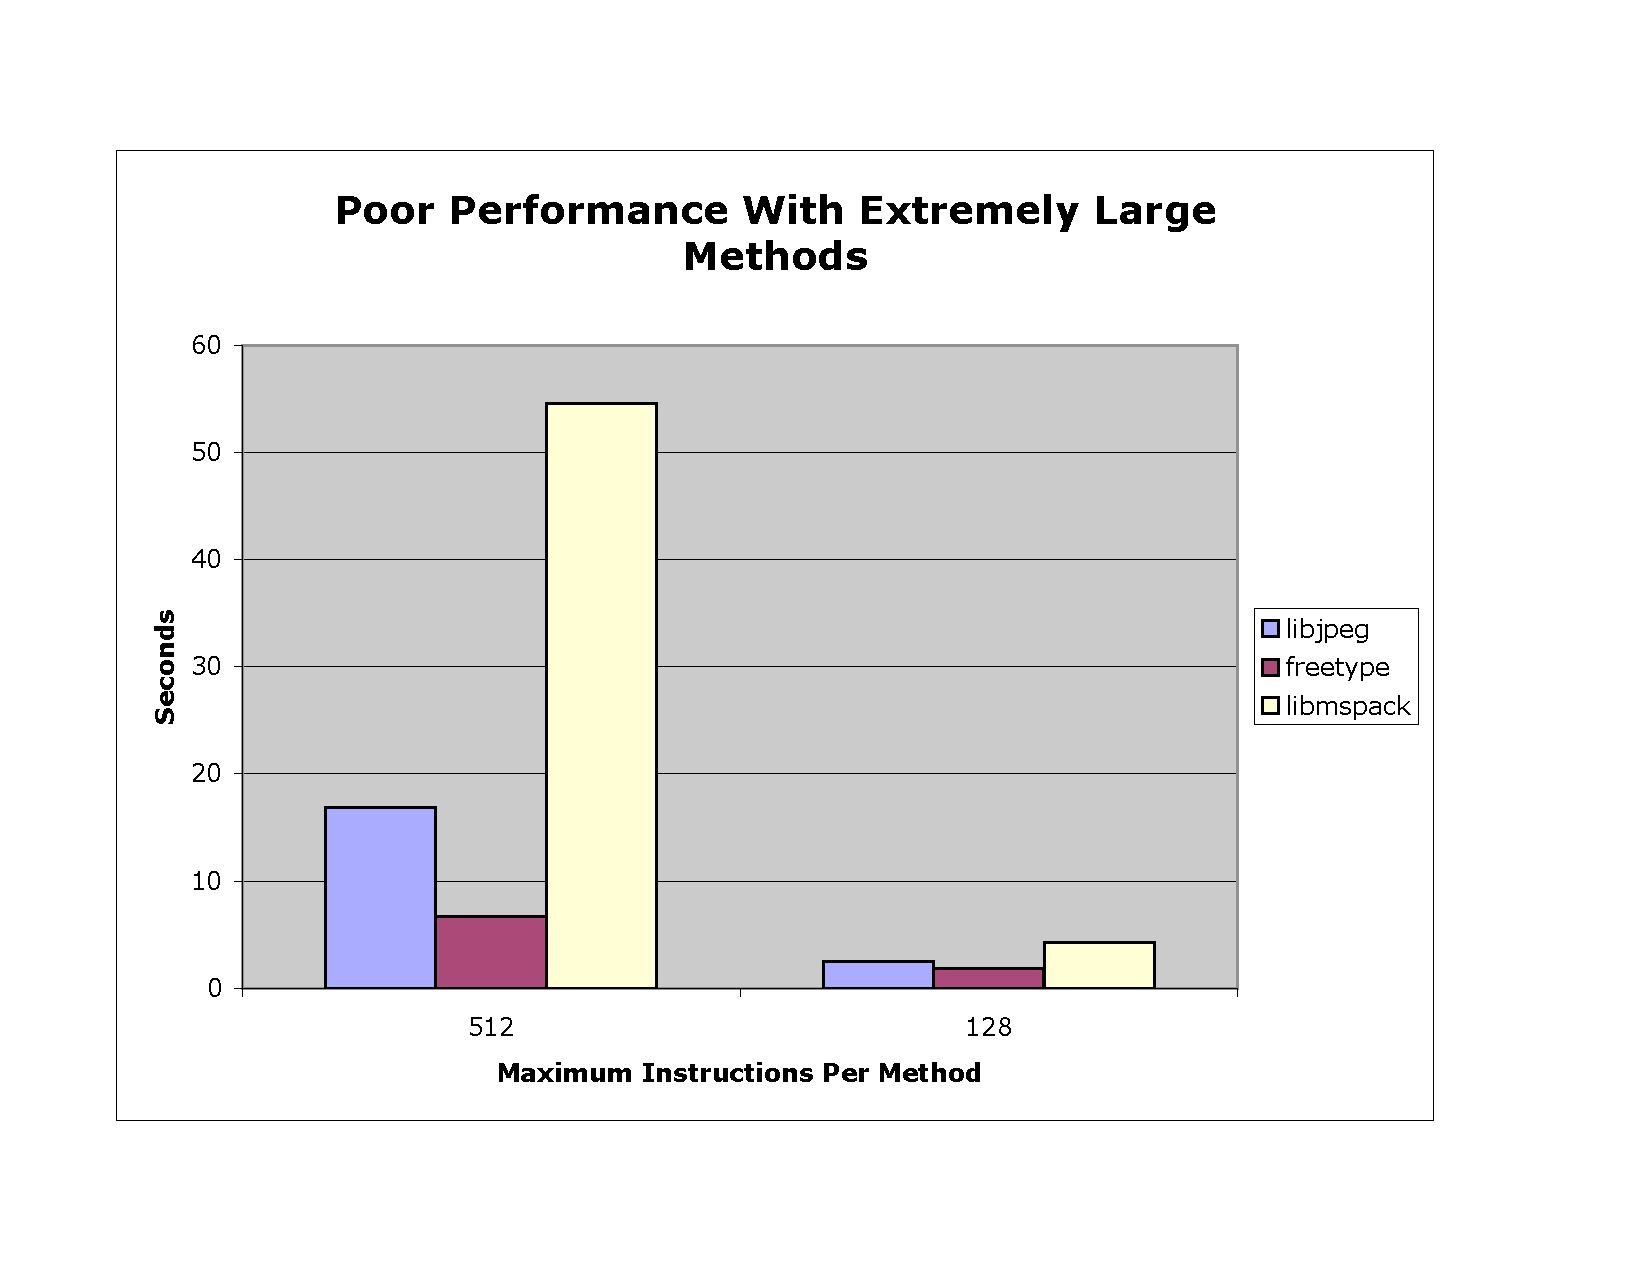
\epsfig{file=chart6,width=\textwidth-1in}
\end{center}
\end{figure}

\end{itemize}


\end{slide}


\begin{slide}\raggedright
\renewcommand{\leftmargini}{5mm}
{\Large{\textcolor{black}{Optimizations: Optimal Method Size}}}
\\\rule{\textwidth}{0.1pt}\\

\begin{itemize}

\item \begin{figure}[H]
\begin{center}
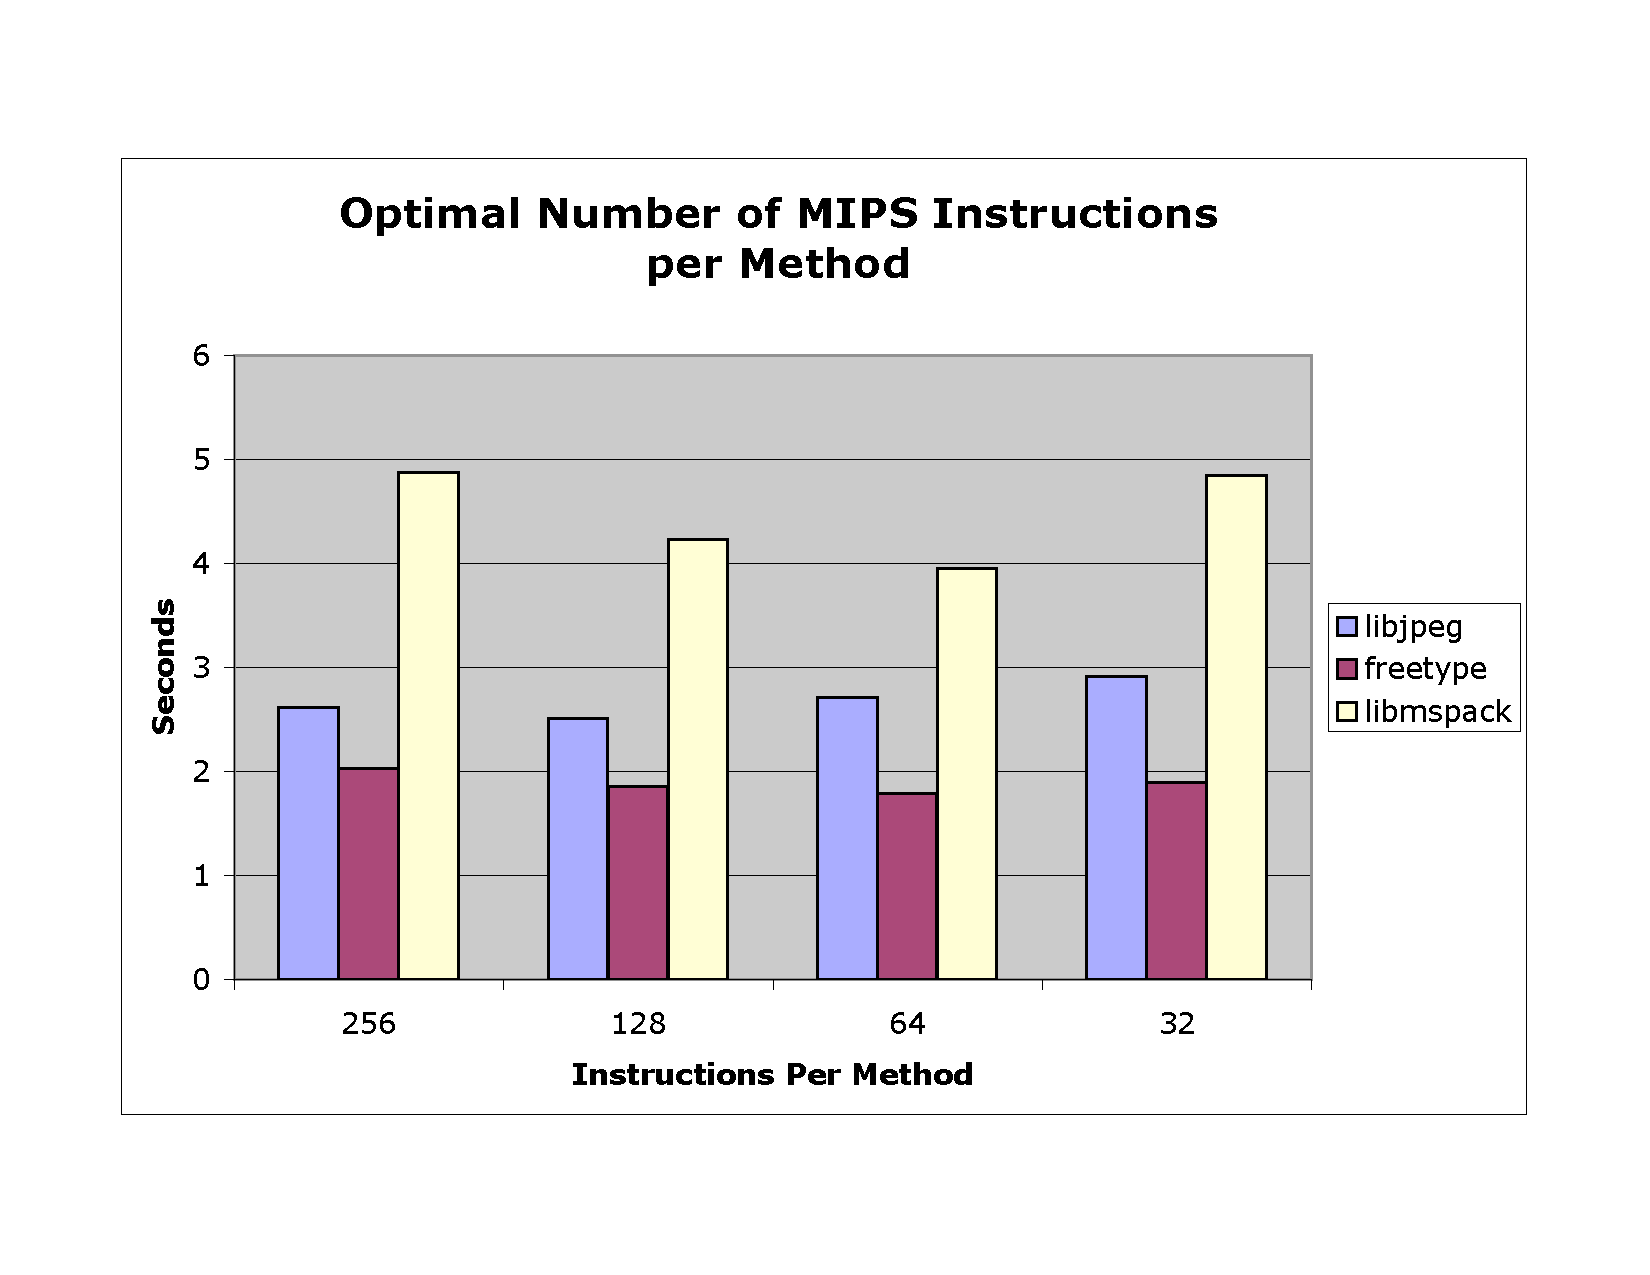
\epsfig{file=chart5,width=\textwidth-1in}
\end{center}
\end{figure}

\end{itemize}


\end{slide}


\begin{slide}\raggedright
\renewcommand{\leftmargini}{5mm}
{\Large{\textcolor{black}{Better Branching}}}
\\\rule{\textwidth}{0.1pt}\\

\begin{itemize}

\item \vspace{5mm}



\begin{Verbatim}[fontsize=\tiny,frame=single,rulecolor=\color{CodeBorder},resetmargins=true,gobble=0]
// Java soucecode
for(;;) {
    switch(pc) {
        case 0x10000: ...
        case 0x10004: // JMP 0x10000
            pc = 0x10000; 
            continue
\end{Verbatim}


\end{itemize}


\end{slide}


\begin{slide}\raggedright
\renewcommand{\leftmargini}{5mm}
{\Large{\textcolor{black}{Better Branching}}}
\\\rule{\textwidth}{0.1pt}\\

\begin{itemize}

\item \vspace{5mm}



\begin{Verbatim}[fontsize=\tiny,frame=single,rulecolor=\color{CodeBorder},resetmargins=true,gobble=0]
// JVM Bytecode
...
10: ...
11: ...
12: GOTO 10 // JMP 0x10000
\end{Verbatim}


\end{itemize}


\end{slide}


\begin{slide}\raggedright
\renewcommand{\leftmargini}{5mm}
{\Large{\textcolor{black}{Better Branching}}}
\\\rule{\textwidth}{0.1pt}\\

\begin{itemize}


\item
     Conditional branches were also not handled optimally in the Binary-
      to-source compiler


\vspace{5mm}



\begin{Verbatim}[fontsize=\tiny,frame=single,rulecolor=\color{CodeBorder},resetmargins=true,gobble=0]
if(condition) {
    pc = 0x10004;
    continue;
}
\end{Verbatim}


\end{itemize}


\end{slide}


\begin{slide}\raggedright
\renewcommand{\leftmargini}{5mm}
{\Large{\textcolor{black}{Better Branching}}}
\\\rule{\textwidth}{0.1pt}\\

\begin{itemize}


\item
     Binary-to-binary compiler emits JVM branch instructions that 
      branch directly to the destination


\vspace{5mm}



\begin{Verbatim}[fontsize=\tiny,frame=single,rulecolor=\color{CodeBorder},resetmargins=true,gobble=0]
...
10: ...
11 ...
12: IFEQ 10
\end{Verbatim}


\end{itemize}


\end{slide}


\begin{slide}\raggedright
\renewcommand{\leftmargini}{5mm}
{\Large{\textcolor{black}{More efficient delay slots}}}
\\\rule{\textwidth}{0.1pt}\\

\begin{itemize}


\item
     The MIPS ISA has ``delay slots'', that is, instruction after a branch instruction 
      that are always executed even if the branch is taken.

\item
     The modification the delay slot makes to the registers used in the branch 
      instruction cannot effect the branch. Therefore, the delay slot cannot just be 
      output before the branch

\item
     In the binary-to-source compiler delay slots were simply output twice (once 
      before setting the new pc and once after the branch)


\end{itemize}


\end{slide}


\begin{slide}\raggedright
\renewcommand{\leftmargini}{5mm}
{\Large{\textcolor{black}{More efficient delay slots}}}
\\\rule{\textwidth}{0.1pt}\\

\begin{itemize}


\item
     The JVM stack can be used to eliminate this inefficiency.

\item
     The variables used in the comparison are pushed to the stack, the 
      delay slot is executed, then the comparison/branch is done

\item
     Delay slot never needs to be output more than once


\end{itemize}


\end{slide}


\begin{slide}\raggedright
\renewcommand{\leftmargini}{5mm}
{\Large{\textcolor{black}{Smaller Bytecode}}}
\\\rule{\textwidth}{0.1pt}\\

\begin{itemize}


\item
     Javac doesn't emit the most space efficient bytecode possible


\vspace{5mm}



\begin{Verbatim}[fontsize=\tiny,frame=single,rulecolor=\color{CodeBorder},resetmargins=true,gobble=0]
switch(pc >>> 8) {
Case 0x1: run_0x100(); break;
Case 0x2: run_0x200(); break;
}
\end{Verbatim}



\item
     Javac emits an ALOAD\_0 and an INVOKESPECIAL instruction for each case arm. 
      The ALOAD\_0 can be hoisted out of the switch statement to create smaller bytecode.



\end{itemize}


\end{slide}


\begin{slide}\raggedright
\renewcommand{\leftmargini}{5mm}
{\Large{\textcolor{black}{Smaller Bytecode}}}
\\\rule{\textwidth}{0.1pt}\\

\begin{itemize}


\item
     Smaller bytecode also results from many of the performance 
      increasing optimizations

\item
     He more efficient branch instructions also take up less space in bytecode

\item
     Using the stack in favor of local variables leads to less LOADs and 
      STORESs

\item
     Better handling of delay slots avoids outputting each delay slot twice


\end{itemize}


\end{slide}


\begin{slide}\raggedright
\renewcommand{\leftmargini}{5mm}
{\Large{\textcolor{black}{GCC Optimizations}}}
\\\rule{\textwidth}{0.1pt}\\

\begin{itemize}


\item
     NestedVM emulates a MIPS R2000 CPU but its performance profile 
      is very different from the actual CPU.

\item
     GCC makes assumptions about the CPU that don't hold true for 
      NestedVM

\item
     This leads to suboptimal code generation


\end{itemize}


\end{slide}


\begin{slide}\raggedright
\renewcommand{\leftmargini}{5mm}
{\Large{\textcolor{black}{GCC Optimizations}}}
\\\rule{\textwidth}{0.1pt}\\

\begin{itemize}


\item
     Fortunately, GCC provides a wealth of options to compensate for 
      this.

\item
     {\texttt{-falign-functions}} - Used to place functions on 512 byte boundaries to 
      reduce the chances of a single function spanning several java 
      methods


\end{itemize}


\end{slide}


\begin{slide}\raggedright
\renewcommand{\leftmargini}{5mm}
{\Large{\textcolor{black}{GCC Optimizations}}}
\\\rule{\textwidth}{0.1pt}\\

\begin{itemize}


\item
     {\texttt{-fno-rename-registers}}

\item
     Normally GCC tries to use as many registers as possible make it easier to 
      schedule code

\item
     This creates more work for the binary translator and the JVM. Using few 
      registers simplifies the resulting bytecode and allows the JIT compiler to 
      better optimize the resulting code.


\end{itemize}


\end{slide}


\begin{slide}\raggedright
\renewcommand{\leftmargini}{5mm}
{\Large{\textcolor{black}{GCC Optimizations}}}
\\\rule{\textwidth}{0.1pt}\\

\begin{itemize}


\item
     {\texttt{-fno-schedule-insns}}

\item
     The results of some MIPS operations are not immediately available. Many 
      instructions have delay slots that are executed before the results are 
      available

\item
     GCC tries to take advantage of these delay slots by using them to do useful 
      work

\item
     Since these results are immediately available in NestedVM this makes the 
      code more complicated with no benefit.


\end{itemize}


\end{slide}


\begin{slide}\raggedright
\renewcommand{\leftmargini}{5mm}
{\Large{\textcolor{black}{Impact of Optimizations}}}
\\\rule{\textwidth}{0.1pt}\\

\begin{itemize}

\item \begin{figure}[H]
\begin{center}
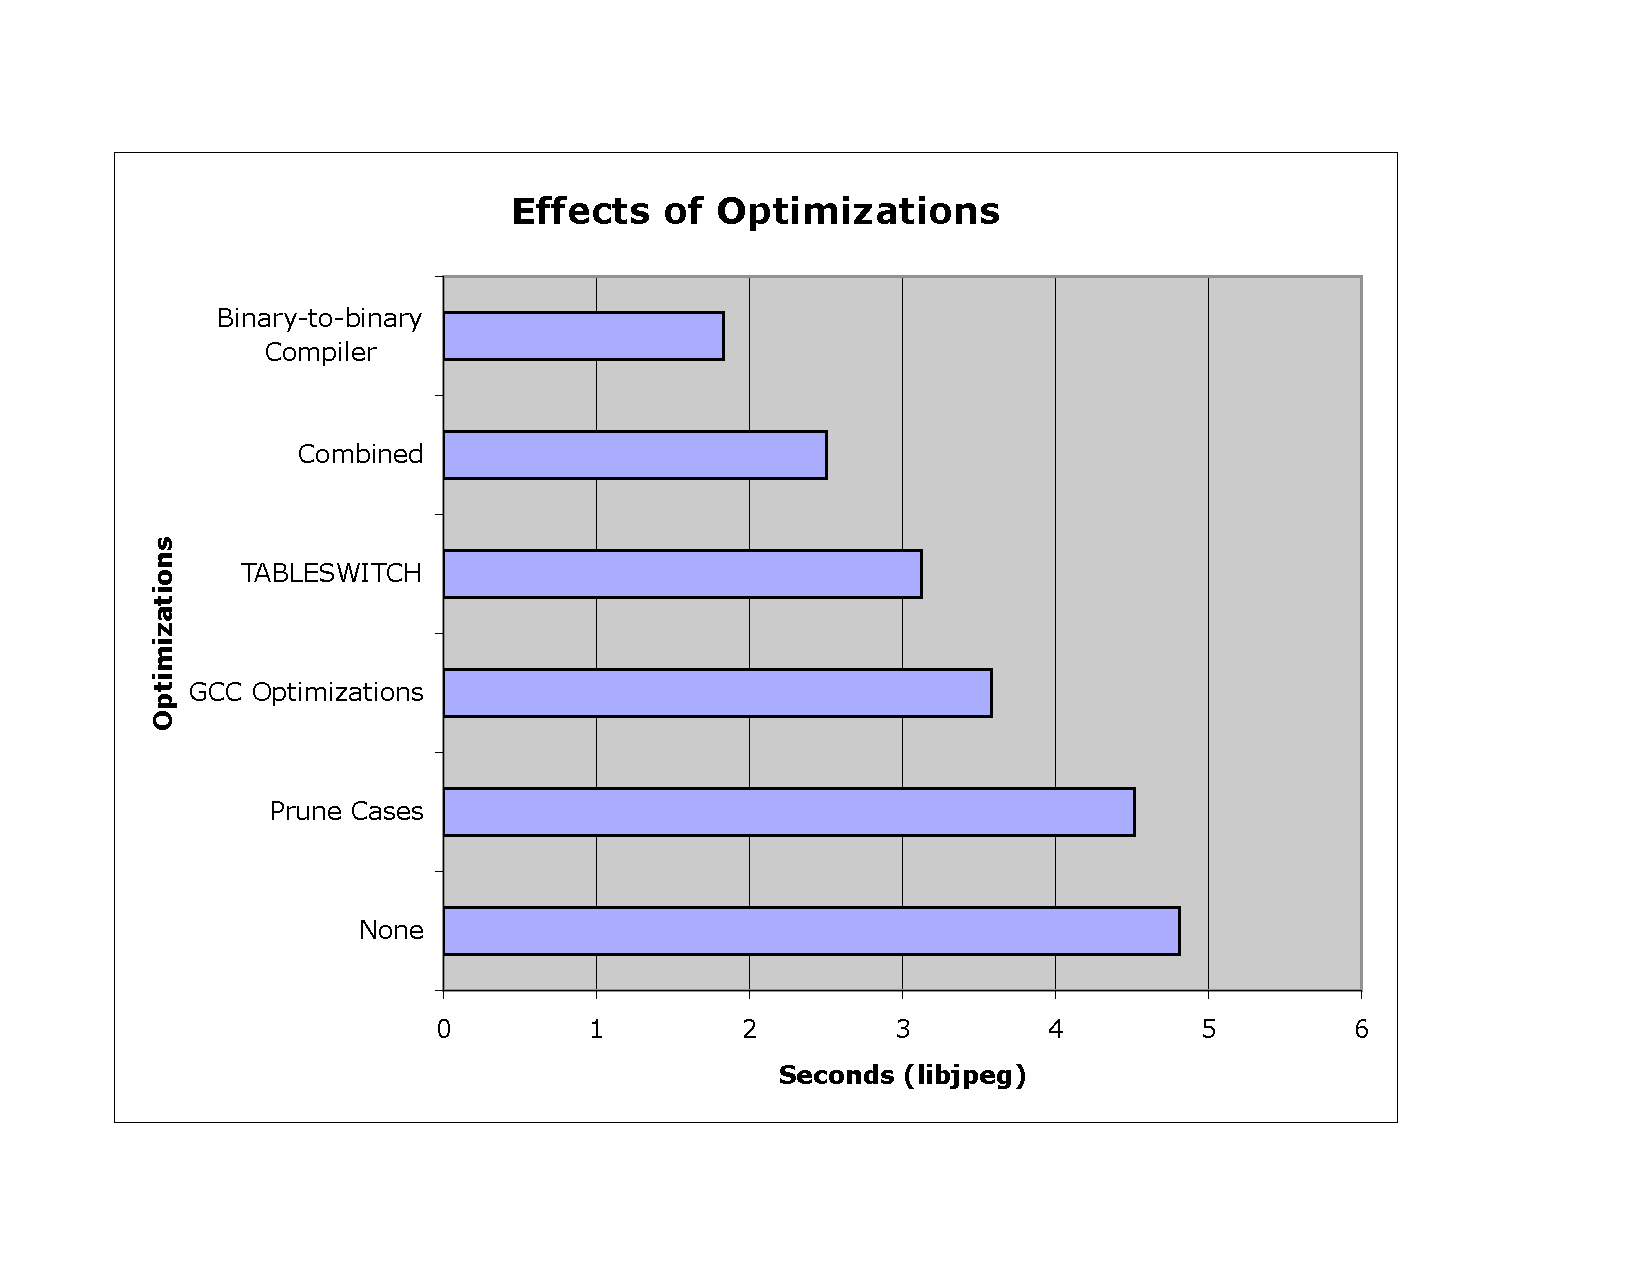
\epsfig{file=chart4,width=\textwidth-1in}
\end{center}
\end{figure}

\end{itemize}


\end{slide}


\begin{slide}\raggedright
\renewcommand{\leftmargini}{5mm}
{\Large{\textcolor{black}{Overall Performance}}}
\\\rule{\textwidth}{0.1pt}\\

\begin{itemize}

\item \begin{figure}[H]
\begin{center}
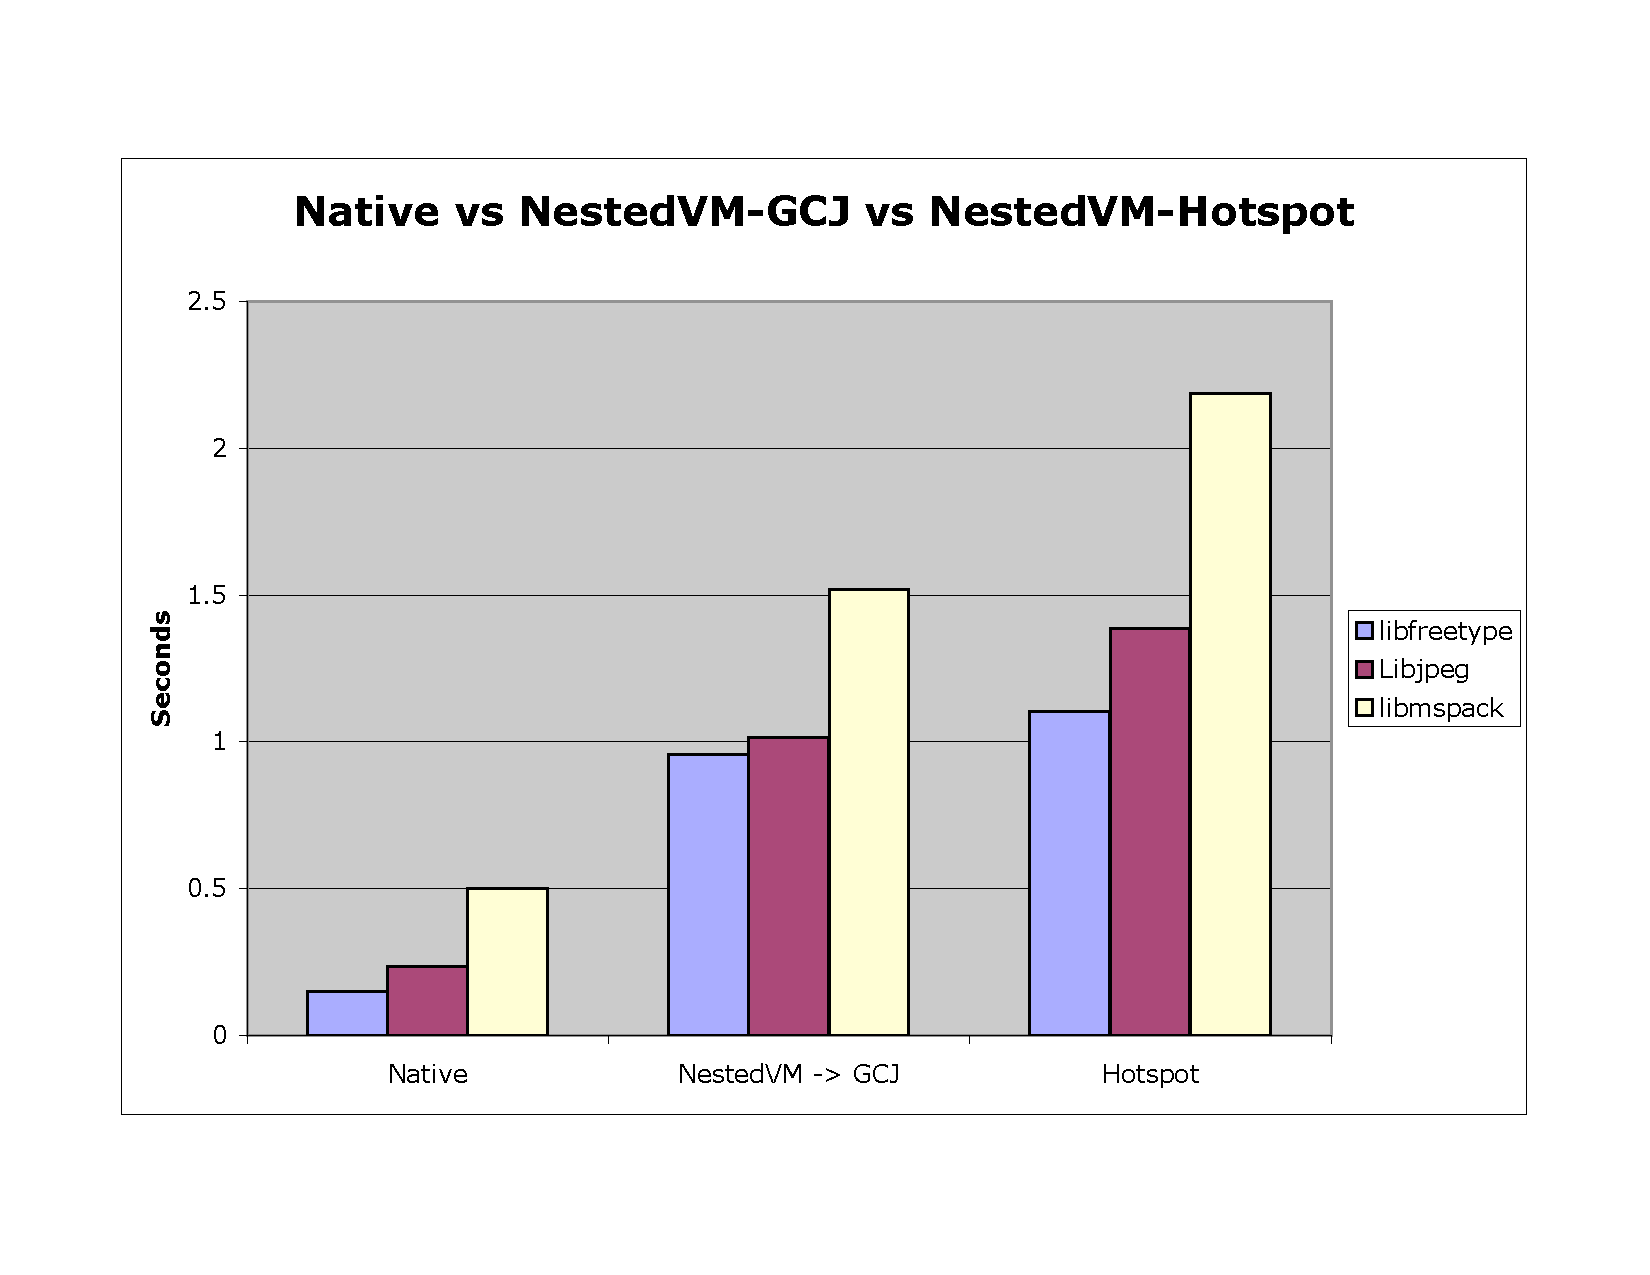
\epsfig{file=chart3,width=\textwidth-1in}
\end{center}
\end{figure}

\end{itemize}


\end{slide}


\begin{slide}\raggedright
\renewcommand{\leftmargini}{5mm}
{\Large{\textcolor{black}{Implementation}}}
\\\rule{\textwidth}{0.1pt}\\

\begin{itemize}


\item
         {\texttt{http://nestedvm.ibex.org/}}
    


\end{itemize}


\end{slide}
\end{document}
